% Select document class: uncomment one of the following
\documentclass[aspectratio=169]{beamer}  % For presentation mode
%\documentclass[11pt]{article}            % For article mode
%\usepackage{beamerarticle}               % Uncomment with article class

% =============================================================================
% COMMON PREAMBLE
% =============================================================================
% =============================================================================
% Common Preamble for Network+ Lecture Series
% This file provides consistent formatting, colors, packages, and styles
% across all lecture modules for both beamer presentations and article mode
% =============================================================================

% =============================================================================
% THEME AND COLORS
% =============================================================================
\usetheme{Madrid}
\usecolortheme{whale}

% Custom colors - standardized across all lectures
\definecolor{rctcblue}{RGB}{0, 74, 136}
\definecolor{rctcgold}{RGB}{255, 199, 44}
\definecolor{networkgreen}{RGB}{0, 128, 64}
\definecolor{alertred}{RGB}{180, 0, 0}
\definecolor{aborange}{RGB}{230, 126, 34}
\definecolor{copperbrown}{RGB}{184, 115, 51}
\definecolor{faborange}{RGB}{255, 165, 0}
\definecolor{fiberyellow}{RGB}{255, 215, 0}
\definecolor{shirepurple}{RGB}{102, 51, 153}
\definecolor{ipblue}{RGB}{52, 152, 219}
\definecolor{ippurple}{RGB}{155, 89, 182}
\definecolor{vlangreen}{RGB}{39, 174, 96}
\definecolor{tcpblue}{RGB}{30, 100, 180}
\definecolor{udpgreen}{RGB}{50, 160, 80}
\definecolor{dhcppurple}{RGB}{120, 60, 160}
\definecolor{dnsyellow}{RGB}{200, 170, 50}
\definecolor{batblack}{RGB}{30, 30, 40}
\definecolor{gothamgray}{RGB}{80, 85, 95}
\definecolor{paddysgreen}{RGB}{19, 77, 33}
\definecolor{beerlight}{RGB}{255, 199, 44}
\definecolor{sunnyorange}{RGB}{255, 140, 0}
\definecolor{ogregreen}{RGB}{34, 139, 34}
\definecolor{swampbrown}{RGB}{101, 67, 33}

% Set theme colors
\setbeamercolor{palette primary}{bg=rctcblue,fg=white}
\setbeamercolor{palette secondary}{bg=rctcblue!80,fg=white}
\setbeamercolor{palette tertiary}{bg=rctcblue!60,fg=white}
\setbeamercolor{structure}{fg=rctcblue}
\setbeamercolor{title}{fg=white,bg=rctcblue}
\setbeamercolor{frametitle}{fg=white,bg=rctcblue}
\setbeamercolor{block title}{bg=rctcblue,fg=white}
\setbeamercolor{block body}{bg=rctcblue!10,fg=black}
\setbeamercolor{block title alerted}{bg=alertred,fg=white}
\setbeamercolor{block body alerted}{bg=alertred!10,fg=black}
\setbeamercolor{block title example}{bg=networkgreen,fg=white}
\setbeamercolor{block body example}{bg=networkgreen!10,fg=black}

% =============================================================================
% PACKAGES
% =============================================================================
\usepackage[utf8]{inputenc}
\usepackage[T1]{fontenc}
\usepackage{lmodern}  % Better font rendering
\usepackage{graphicx}
\usepackage{tikz}
\usepackage{booktabs}
\usepackage{array}
\usepackage{multirow}
\usepackage{hyperref}
\usepackage{adjustbox}
\usepackage{amssymb}
\usepackage{amsmath}
\usepackage{calc}
\usepackage{fontawesome5}
% xcolor with [table] option: avoid colortbl.4ht hook conflict in tex4ht
\ifdefined\HCode
  \usepackage{xcolor}
  \usepackage{colortbl}  % provides \rowcolor etc.
\else
  \usepackage[table]{xcolor}  % includes colortbl for pdflatex
\fi

% =============================================================================
% TIKZ LIBRARIES AND SETUP
% =============================================================================
\usetikzlibrary{
    shapes.geometric,
    shapes.symbols,
    shapes.misc,
    arrows.meta,
    positioning,
    calc,
    fit,
    backgrounds,
    decorations.pathreplacing,
    decorations.pathmorphing,
    matrix,
    chains
}
% shadows library causes pgfuseshading errors with tex4ht;
% only load it when NOT building HTML
\ifdefined\HCode\else
    \usetikzlibrary{shadows}
\fi

% Graphics path for icons and chapter images
\graphicspath{
    {../images/icons/}
    {./images/icons/}
    {images/icons/}
    {../images/ch1/}
    {./images/ch1/}
    {images/ch1/}
    {../images/ch2/}
    {./images/ch2/}
    {images/ch2/}
    {../images/ch3/}
    {./images/ch3/}
    {images/ch3/}
    {../images/ch4/}
    {./images/ch4/}
    {images/ch4/}
    {../images/ch5/}
    {./images/ch5/}
    {images/ch5/}
    {../images/ch6/}
    {./images/ch6/}
    {images/ch6/}
    {../images/ch7/}
    {./images/ch7/}
    {images/ch7/}
    {../images/ch8/}
    {./images/ch8/}
    {images/ch8/}
    {../images/ch9/}
    {./images/ch9/}
    {images/ch9/}
    {../images/}
    {./images/}
    {images/}
}

% =============================================================================
% NETWORK DIAGRAM STYLES
% =============================================================================
\tikzset{
    % Node styles for network devices
    device/.style={
        inner sep=2pt,
        label distance=2pt
    },
    pc/.style={device},
    laptop/.style={device},
    server/.style={device},
    router/.style={device},
    switch/.style={device},
    firewall/.style={device},
    cloud/.style={device},
    phone/.style={device},
    tablet/.style={device},
    wifi/.style={device},
    % Connection styles
    ethernet/.style={
        draw=rctcblue,
        line width=1.5pt,
        -{Stealth[length=3mm]}
    },
    ethernet noarrow/.style={
        draw=rctcblue,
        line width=1.5pt
    },
    wireless/.style={
        draw=aborange,
        line width=1.5pt,
        dashed,
        -{Stealth[length=3mm]}
    },
    wireless noarrow/.style={
        draw=aborange,
        line width=1.5pt,
        dashed
    },
    wan/.style={
        draw=alertred,
        line width=2pt,
        -{Stealth[length=3mm]}
    },
    wan noarrow/.style={
        draw=alertred,
        line width=2pt
    },
    copper/.style={
        draw=copperbrown,
        line width=2pt,
        -{Stealth[length=3mm]}
    },
    copper noarrow/.style={
        draw=copperbrown,
        line width=2pt
    },
    fiber/.style={
        draw=fiberyellow,
        line width=2pt,
        -{Stealth[length=3mm]}
    },
    fiber noarrow/.style={
        draw=fiberyellow,
        line width=2pt
    },
    trunk/.style={
        draw=shirepurple,
        line width=2pt,
        -{Stealth[length=3mm]}
    },
    trunk noarrow/.style={
        draw=shirepurple,
        line width=2pt
    },
    % Packet/segment styles
    pktseg/.style={
        draw=rctcblue,
        fill=rctcblue!10,
        minimum height=0.5cm,
        font=\tiny,
        rounded corners=2pt
    },
    pktseg tcp/.style={
        draw=tcpblue,
        fill=tcpblue!15,
        minimum height=0.5cm,
        font=\tiny,
        rounded corners=2pt
    },
    pktseg udp/.style={
        draw=udpgreen,
        fill=udpgreen!15,
        minimum height=0.5cm,
        font=\tiny,
        rounded corners=2pt
    },
    pktseg highlight/.style={
        draw=aborange,
        fill=aborange!20,
        minimum height=0.5cm,
        font=\tiny,
        rounded corners=2pt
    },
    % Box styles
    ipbox/.style={
        draw=rctcblue,
        fill=rctcblue!10,
        rounded corners,
        minimum height=0.4cm,
        font=\small
    },
    portbox/.style={
        draw=tcpblue,
        fill=tcpblue!10,
        rounded corners,
        minimum height=0.4cm,
        font=\small
    },
    dnsbox/.style={
        draw=dnsyellow,
        fill=dnsyellow!15,
        rounded corners,
        minimum height=0.4cm,
        font=\small
    },
    routetable/.style={
        draw=rctcblue,
        fill=rctcblue!10,
        rounded corners,
        minimum height=0.4cm,
        font=\small
    },
    macbox/.style={
        draw=networkgreen,
        fill=networkgreen!10,
        rounded corners,
        minimum height=0.4cm,
        font=\small
    },
    % Frame segment styles (Ethernet frame diagrams)
    frameseg/.style={
        draw=rctcblue,
        fill=rctcblue!10,
        minimum height=0.5cm,
        font=\tiny,
        rounded corners=2pt
    },
    frameseg highlight/.style={
        draw=aborange,
        fill=aborange!20,
        minimum height=0.5cm,
        font=\tiny,
        rounded corners=2pt
    },
    % Process/flow styles
    process/.style={
        draw=rctcblue,
        fill=rctcblue!15,
        rounded corners,
        minimum width=2cm,
        minimum height=0.6cm,
        font=\small,
        align=center
    },
    decision/.style={
        draw=aborange,
        fill=aborange!15,
        diamond,
        aspect=2,
        minimum width=1.5cm,
        font=\small,
        align=center
    },
    % OSI Layer styles
    osilayer/.style={
        draw=rctcblue,
        fill=rctcblue!10,
        minimum width=3cm,
        minimum height=0.45cm,
        font=\small
    },
    osilayer highlight/.style={
        draw=aborange,
        fill=aborange!20,
        line width=1.5pt,
        minimum width=3cm,
        minimum height=0.45cm,
        font=\small\bfseries
    }
}

% =============================================================================
% ICON COMMANDS - Standardized using PNG files and FontAwesome
% =============================================================================
% Network device icons (PNG)
\newcommand{\iconpc}[1][0.6cm]{\resizebox{#1}{!}{
\includegraphics{icon_pc}}}
\newcommand{\iconlaptop}[1][0.6cm]{\resizebox{#1}{!}{
\includegraphics{icon_laptop}}}
\newcommand{\iconserver}[1][0.6cm]{\resizebox{#1}{!}{
\includegraphics{icon_server}}}
\newcommand{\iconrouter}[1][0.6cm]{\resizebox{#1}{!}{
\includegraphics{icon_router}}}
\newcommand{\iconswitch}[1][0.6cm]{\resizebox{#1}{!}{
\includegraphics{icon_switch}}}
\newcommand{\iconfirewall}[1][0.6cm]{\resizebox{#1}{!}{
\includegraphics{icon_firewall}}}
\newcommand{\iconcloud}[1][0.6cm]{\resizebox{#1}{!}{
\includegraphics{icon_cloud}}}
\newcommand{\iconphone}[1][0.6cm]{\resizebox{#1}{!}{
\includegraphics{icon_phone}}}
\newcommand{\icontablet}[1][0.6cm]{\resizebox{#1}{!}{
\includegraphics{icon_tablet}}}
\newcommand{\iconwifi}[1][0.6cm]{\resizebox{#1}{!}{
\includegraphics{icon_wifi}}}
\newcommand{\icondatabase}[1][0.6cm]{\resizebox{#1}{!}{
\includegraphics{icon_db}}}
\newcommand{\iconlock}[1][0.6cm]{\resizebox{#1}{!}{
\includegraphics{icon_lock}}}

% For HTML/tex4ht builds: replace PNG icons with FontAwesome5 glyphs.
% dvisvgm embeds font glyphs as vectors but silently ignores em:graph (PNG)
% specials, so PNG icons would be blank in the output SVGs. FA5 glyphs work.
\ifdefined\HCode
  \renewcommand{\iconpc}[1][0.6cm]{\resizebox{#1}{!}{\faIcon{desktop}}}
  \renewcommand{\iconlaptop}[1][0.6cm]{\resizebox{#1}{!}{\faIcon{laptop}}}
  \renewcommand{\iconserver}[1][0.6cm]{\resizebox{#1}{!}{\faIcon{server}}}
  \renewcommand{\iconrouter}[1][0.6cm]{\resizebox{#1}{!}{\faIcon{route}}}
  \renewcommand{\iconswitch}[1][0.6cm]{\resizebox{#1}{!}{\faIcon{network-wired}}}
  \renewcommand{\iconfirewall}[1][0.6cm]{\resizebox{#1}{!}{\faIcon{shield-alt}}}
  \renewcommand{\iconcloud}[1][0.6cm]{\resizebox{#1}{!}{\faIcon{cloud}}}
  \renewcommand{\iconphone}[1][0.6cm]{\resizebox{#1}{!}{\faIcon{mobile-alt}}}
  \renewcommand{\icontablet}[1][0.6cm]{\resizebox{#1}{!}{\faIcon{tablet-alt}}}
  \renewcommand{\iconwifi}[1][0.6cm]{\resizebox{#1}{!}{\faIcon{wifi}}}
  \renewcommand{\icondatabase}[1][0.6cm]{\resizebox{#1}{!}{\faIcon{database}}}
  \renewcommand{\iconlock}[1][0.6cm]{\resizebox{#1}{!}{\faIcon{lock}}}
\fi

% FontAwesome icons
\newcommand{\iconuser}[1][0.6cm]{\resizebox{#1}{!}{\faIcon{user}}}
\newcommand{\iconglobe}[1][0.6cm]{\resizebox{#1}{!}{\faIcon{globe}}}
\newcommand{\iconclock}[1][0.6cm]{\resizebox{#1}{!}{\faIcon{clock}}}
\newcommand{\iconmail}[1][0.6cm]{\resizebox{#1}{!}{\faIcon{envelope}}}
\newcommand{\icondoc}[1][0.6cm]{\resizebox{#1}{!}{\faIcon{file-alt}}}
\newcommand{\iconsearch}[1][0.6cm]{\resizebox{#1}{!}{\faIcon{search}}}
\newcommand{\icontools}[1][0.6cm]{\resizebox{#1}{!}{\faIcon{tools}}}
\newcommand{\iconchart}[1][0.6cm]{\resizebox{#1}{!}{\faIcon{chart-line}}}
\newcommand{\iconalert}[1][0.6cm]{\resizebox{#1}{!}{\faIcon{bell}}}
\newcommand{\iconlog}[1][0.6cm]{\resizebox{#1}{!}{\faIcon{clipboard-list}}}
\newcommand{\iconeye}[1][0.6cm]{\resizebox{#1}{!}{\faIcon{eye}}}
\newcommand{\iconhacker}[1][0.6cm]{\resizebox{#1}{!}{\faIcon{user-secret}}}
\newcommand{\iconkey}[1][0.6cm]{\resizebox{#1}{!}{\faIcon{key}}}
\newcommand{\iconfile}[1][0.6cm]{\resizebox{#1}{!}{\faIcon{file-alt}}}
\newcommand{\icondog}[1][0.6cm]{\resizebox{#1}{!}{\faIcon{dog}}}
\newcommand{\iconcat}[1][0.6cm]{\resizebox{#1}{!}{\faIcon{cat}}}
\newcommand{\iconvoip}[1][0.6cm]{\resizebox{#1}{!}{\faIcon{phone-volume}}}
\newcommand{\iconmoney}[1][0.6cm]{\resizebox{#1}{!}{\faIcon{money-bill-wave}}}
\newcommand{\icontrash}[1][0.6cm]{\resizebox{#1}{!}{\faIcon{trash}}}
\newcommand{\iconbuilding}[1][0.6cm]{\resizebox{#1}{!}{\faIcon{building}}}

% =============================================================================
% CUSTOM COMMANDS AND ENVIRONMENTS
% =============================================================================

% Key term formatting
\newcommand{\keyterm}[1]{\textbf{#1}}

% Slide section marker
\newcommand{\sectionslide}[1]{
    \begin{frame}
        \vfill
        \centering
        \begin{beamercolorbox}[sep=8pt,center,shadow=true,rounded=true]{title}
            \usebeamerfont{title}\Huge #1
        \end{beamercolorbox}
        \vfill
    \end{frame}
}

% Case study frame environment
\newenvironment{casestudy}[1]{%
    \begin{alertblock}{$\blacktriangleright$ Case Study: #1}
}{%
    \end{alertblock}
}

% Solution frame environment  
\newenvironment{casesolution}[1]{%
    \begin{exampleblock}{$\checkmark$ Solution: #1}
}{%
    \end{exampleblock}
}

% =============================================================================
% FOOTER WITH SLIDE NUMBERS
% =============================================================================
\setbeamertemplate{footline}{
    \leavevmode%
    \hbox{%
        \begin{beamercolorbox}[wd=.333333\paperwidth,ht=2.25ex,dp=1ex,center]{author in head/foot}%
            \usebeamerfont{author in head/foot}\insertshortauthor
        \end{beamercolorbox}%
        \begin{beamercolorbox}[wd=.333333\paperwidth,ht=2.25ex,dp=1ex,center]{title in head/foot}%
            \usebeamerfont{title in head/foot}\insertshorttitle
        \end{beamercolorbox}%
        \begin{beamercolorbox}[wd=.333333\paperwidth,ht=2.25ex,dp=1ex,right]{date in head/foot}%
            \usebeamerfont{date in head/foot}\insertshortdate{}\hspace*{2em}
            \insertframenumber{} / \inserttotalframenumber\hspace*{2ex}
        \end{beamercolorbox}}%
    \vskip0pt%
}

% =============================================================================
% ARTICLE MODE SUPPORT
% =============================================================================
% The following commands help with beamerarticle mode for HTML conversion

% In article mode, add proper section/subsection support and override environments
\mode<article>{
    % Make sure figure captions work properly
    \setbeamertemplate{caption}[numbered]
    \setbeamertemplate{caption label separator}{: }
    
    % Add some spacing for readability
    \setlength{\parskip}{0.5em}
    \setlength{\parindent}{0pt}
    
    % Article mode versions of case study environments
    \renewenvironment{casestudy}[1]{%
        \vspace{0.3cm}\noindent\textbf{Case Study: #1}\newline\begin{itshape}
    }{%
        \end{itshape}\vspace{0.3cm}
    }
    
    \renewenvironment{casesolution}[1]{%
        \vspace{0.3cm}\noindent\textbf{Solution: #1}\newline\begin{itshape}
    }{%
        \end{itshape}\vspace{0.3cm}
    }
}

% Command to mark content that only appears in article mode
\newcommand{\articleonly}[1]{\mode<article>{#1}}

% Command to mark content that only appears in presentation mode
\newcommand{\presentationonly}[1]{\mode<presentation>{#1}}


% =============================================================================
% DOCUMENT INFO
% =============================================================================
\title[Zones, IoT, and Physical Security]{Module 11: Zone-Based Security, IoT, and Physical Security}
\subtitle{Intro to Networks}
\author{Brendan Shea, PhD}
\institute{Rochester Community and Technical College}
\date{}

\begin{document}

% =============================================================================
% Module 11: Zone-Based Security, IoT, and Physical Security
% =============================================================================

\begin{frame}
    \titlepage
    \begin{center}
        \begin{tikzpicture}[scale=0.85]
            % Nested zone rings: Internet -> DMZ -> Internal
            \draw[thick, alertred, fill=alertred!8] (0,0) ellipse (3.2cm and 1.1cm);
            \node[font=\tiny, text=alertred] at (2.5, 0.65) {Internet};
            \draw[thick, aborange, fill=aborange!15] (0,0) ellipse (2.1cm and 0.75cm);
            \node[font=\tiny, text=aborange] at (0, 0.5) {DMZ};
            \draw[thick, networkgreen, fill=networkgreen!20] (0,0) ellipse (1.1cm and 0.4cm);
            \node[font=\tiny, text=networkgreen] at (0, 0) {Internal};
            % Firewall icons
            \node (fw1) at (-3.6, 0) {\faIcon{shield-alt}};
            \node[below=0.05cm of fw1, font=\tiny] {Outer FW};
            \node (fw2) at (-1.5, 0) {\faIcon{shield-alt}};
            \node[below=0.05cm of fw2, font=\tiny] {Inner FW};
        \end{tikzpicture}
    \end{center}
\end{frame}

\presentationonly{
\begin{frame}[allowframebreaks]{Outline}
\small
\tableofcontents[hideallsubsections]
\end{frame}
}

% =============================================================================
\section*{Review from Module 10}
% =============================================================================

\begin{frame}{Review: Identity, Access, and Hardening}
    \begin{columns}[T]
        \begin{column}{0.48\textwidth}
            \begin{block}{Key Module 10 Ideas}
                \begin{itemize}
                    \item \textbf{AAA}: Authenticate who you are, authorize what you can do, and account for what you did.
                    \item \textbf{RBAC and least privilege}: users and services should only have access to exactly what they need.
                    \item \textbf{Hardening}: Remove defaults, disable unused services, patch regularly.
                    \item \textbf{ACLs and firewalls}: Enforce traffic policy at network boundaries.
                \end{itemize}
            \end{block}
        \end{column}
        \begin{column}{0.48\textwidth}
            \begin{alertblock}{Where Module 11 Takes This}
                Module 10 controlled \emph{who} gets access. Module 11 controls \emph{where} traffic is allowed to travel, how \textbf{physical zones} enforce security, and why devices like medical monitors and building sensors need special network treatment.
            \end{alertblock}
        \end{column}
    \end{columns}
\end{frame}

% =============================================================================
\section*{Learning Outcomes}
% =============================================================================

\begin{frame}[t,allowframebreaks]{Learning Outcomes}
    After completing this module, you will be able to:
    \vspace{0.5em}
    \small
    \begin{itemize}
        \item Describe \keyterm{network security zones} and explain why separating traffic by trust level reduces risk.
        \item Define the \keyterm{screened subnet} (DMZ) and identify which services belong inside it.
        \item Explain the role of \keyterm{perimeter networks} and how dual-firewall architectures differ from single-firewall designs.
        \item Identify common \keyterm{IoT device} categories and explain why they present unique security challenges.
        \item Describe \keyterm{industrial and embedded systems} and their constraints (long lifecycles, no patch support, safety-critical operation).
        \item Explain how to segment IoT devices onto isolated networks to limit their attack surface.
        \item Describe physical security controls: locks, access cards, mantraps, cameras, and motion sensors.
        \item Explain \keyterm{geofencing} and how location-based policies complement network controls.
        \item Apply defense-in-depth thinking across all three domains: logical zones, device segmentation, and physical access.
    \end{itemize}
\end{frame}

% =============================================================================
\section{Zone-Based Security}
\subsection{Network Security Zones}
% =============================================================================

\articleonly{
This section introduces the concept of network security zones, explains the architecture of screened subnets (DMZs) and perimeter networks, and covers how to design layered perimeter defenses.
}

% --- NEW SLIDE ---
\begin{frame}{11.1 Zone-Based Security: The Big Idea}
    \footnotesize
    Not all traffic deserves equal trust. \keyterm{Zone-based security} divides a network into distinct areas with defined trust levels, and enforces rules about which zones can talk to each other.

    \vspace{0.4em}
    \begin{exampleblock}{Hospital Floor Analogy}
        \footnotesize
        Think about how a hospital manages access to different spaces:
        \begin{itemize}
            \item \textbf{Public lobby}: Anyone can walk in --- untrusted, uncontrolled.
            \item \textbf{Emergency department}: Patients and staff only, ID required.
            \item \textbf{ICU}: Authorized clinical staff only, strict access log.
            \item \textbf{Operating theater}: Only the surgical team, sterile protocol.
        \end{itemize}
        Network zones work the same way. You do not give a visitor the same access as a surgeon.
    \end{exampleblock}

    \begin{block}{Why zones matter}
        \footnotesize
        If everything is on one flat network, a compromised device anywhere can reach everything everywhere. Zones \textbf{contain} breaches and \textbf{limit blast radius}.
    \end{block}
\end{frame}

% --- NEW SLIDE ---
\begin{frame}{Network Security Zones}
    \footnotesize
    Most enterprise and healthcare networks organize traffic into at least three logical zones based on trust level.

    \vspace{0.3em}
    \begin{columns}[T]
        \begin{column}{0.32\textwidth}
            \begin{alertblock}{Untrusted (Internet)}
                \footnotesize
                The public internet. \textbf{Trust level: zero.} Traffic is assumed hostile until proven otherwise.
            \end{alertblock}
        \end{column}
        \begin{column}{0.32\textwidth}
            \begin{block}{Semi-Trusted (DMZ)}
                \footnotesize
                Services that must be reachable from the internet but should \emph{not} have direct access to internal systems. Web servers, email gateways, patient portals.
            \end{block}
        \end{column}
        \begin{column}{0.32\textwidth}
            \begin{exampleblock}{Trusted (Internal)}
                \footnotesize
                Workstations, EHR servers, file servers, medical devices. Should \textbf{never} be directly reachable from the internet.
            \end{exampleblock}
        \end{column}
    \end{columns}

    \vspace{0.3em}
    \begin{alertblock}{Medical IT: A Fourth Zone}
        \footnotesize
        Many healthcare environments add a dedicated \textbf{clinical/biomedical zone} for networked patient-care devices (infusion pumps, monitors, imaging). These devices often cannot be patched --- isolating them limits exposure even if a workstation elsewhere is compromised.
    \end{alertblock}
\end{frame}

% --- NEW SLIDE ---
\begin{frame}{Zone Policies: What Is Allowed Between Zones?}
    \footnotesize
    Zones are only useful if you enforce policies at the boundaries. Default policy is \textbf{deny}; only explicitly permitted traffic passes.

    \vspace{0.3em}
    \begin{table}[]
        \renewcommand{\arraystretch}{1.3}
        \centering
        \small
        \begin{tabular}{|l|l|l|}
        \hline
        \rowcolor[HTML]{EFEFEF} \textbf{From} & \textbf{To} & \textbf{Typical Policy} \\ \hline
        Internet & DMZ & Permit only: HTTP/S, SMTP (inbound mail) \\ \hline
        Internet & Internal & \textbf{Deny all} (no exceptions) \\ \hline
        DMZ & Internal & Deny by default; permit only specific DB queries \\ \hline
        Internal & DMZ & Permit outbound to published services \\ \hline
        Internal & Internet & Permit outbound; filtered by proxy \\ \hline
        Clinical zone & Internal EHR & Permit only EHR data flow ports \\ \hline
        \end{tabular}
    \end{table}

    \begin{block}{Key rule}
        \footnotesize
        Traffic from a \emph{lower}-trust zone to a \emph{higher}-trust zone must always be explicitly justified and tightly scoped. A DMZ web server should never freely connect to an internal file server.
    \end{block}
\end{frame}

% =============================================================================
\subsection{Screened Subnets and the DMZ}
% =============================================================================

% --- NEW SLIDE ---
\begin{frame}{Configuring a Screened Subnet}
    \footnotesize
    A \keyterm{screened subnet} (also called a \keyterm{DMZ} --- demilitarized zone) is a network segment sandwiched between two firewalls: one facing the internet, one facing the internal network.

    \vspace{0.3em}
    \begin{columns}[T]
        \begin{column}{0.52\textwidth}
            \begin{block}{Dual-Firewall Architecture}
                \footnotesize
                \begin{enumerate}
                    \item \textbf{Outer firewall}: Faces the internet. Allows inbound traffic only to services in the DMZ.
                    \item \textbf{DMZ}: Hosts services that must be reachable externally (web, email, VPN).
                    \item \textbf{Inner firewall}: Protects the internal network. DMZ hosts cannot initiate connections to internal servers unless explicitly permitted.
                \end{enumerate}
            \end{block}
            \begin{alertblock}{Why two firewalls?}
                \footnotesize
                If the outer firewall is compromised, the inner firewall still protects internal systems. A single-firewall DMZ (three-legged) is cheaper but offers less isolation.
            \end{alertblock}
        \end{column}
        \begin{column}{0.44\textwidth}
            \begin{center}
                \begin{tikzpicture}[scale=0.72]
                    \node (inet) at (0, 4.5) {\faIcon{globe}};
                    \node[font=\tiny] at (0, 4.0) {Internet};
                    \node (fw1) at (0, 3.2) {\faIcon{shield-alt}};
                    \node[font=\tiny, right] at (0.25, 3.2) {Outer Firewall};
                    \node[draw, fill=aborange!20, rounded corners, minimum width=2.2cm, minimum height=0.7cm] (dmz) at (0, 2.1) {};
                    \node[font=\tiny] at (0, 2.1) {DMZ (Web, Email, VPN)};
                    \node (fw2) at (0, 1.0) {\faIcon{shield-alt}};
                    \node[font=\tiny, right] at (0.25, 1.0) {Inner Firewall};
                    \node[draw, fill=networkgreen!20, rounded corners, minimum width=2.2cm, minimum height=0.7cm] (internal) at (0, 0) {};
                    \node[font=\tiny] at (0, 0) {Internal Network};
                    \draw[->, thick] (inet) -- (fw1);
                    \draw[->, thick] (fw1) -- (dmz);
                    \draw[->, thick] (dmz) -- (fw2);
                    \draw[->, thick] (fw2) -- (internal);
                \end{tikzpicture}
            \end{center}
        \end{column}
    \end{columns}
\end{frame}

\articleonly{
\par\small\emph{The screened subnet diagram shows the dual-firewall architecture. Traffic from the Internet first hits the Outer Firewall, which permits only specific inbound services into the DMZ (web, email, VPN). A second Inner Firewall sits between the DMZ and the Internal Network. Even if an attacker compromises a DMZ host, they still face the inner firewall before reaching internal systems. This defense-in-depth principle means two independent security controls must both fail for an attacker to reach the trusted network.}\par
}

% --- NEW SLIDE ---
\begin{frame}{Perimeter Networks}
    \footnotesize
    A \keyterm{perimeter network} is the broader concept of a defended boundary between zones --- the DMZ is its most common implementation.

    \vspace{0.3em}
    \begin{columns}[T]
        \begin{column}{0.48\textwidth}
            \begin{block}{What Belongs on the Perimeter?}
                \footnotesize
                \begin{itemize}
                    \item \textbf{Web / application servers}: Serve external users.
                    \item \textbf{Email gateway / spam filter}: Processes inbound mail before delivery.
                    \item \textbf{VPN concentrator}: Terminates remote-access tunnels.
                    \item \textbf{Reverse proxy}: Forwards external HTTP requests to internal app servers.
                    \item \textbf{Patient portal servers}: Public-facing; must \emph{not} share a segment with the EHR backend.
                \end{itemize}
            \end{block}
        \end{column}
        \begin{column}{0.48\textwidth}
            \begin{alertblock}{What Does NOT Belong on the Perimeter?}
                \footnotesize
                \begin{itemize}
                    \item Internal file servers, AD domain controllers
                    \item EHR / clinical databases
                    \item Medical devices (infusion pumps, monitors)
                    \item HR, payroll, financial systems
                \end{itemize}
                \vspace{0.2em}
                If a DMZ host is compromised, anything on the same segment is directly exposed.
            \end{alertblock}
        \end{column}
    \end{columns}
\end{frame}

% --- NEW SLIDE ---
\begin{frame}{Screened Subnets: Design Choices}
    \footnotesize
    Organizations can implement screened subnets in several ways, each with trade-offs.

    \vspace{0.3em}
    \begin{table}[]
        \renewcommand{\arraystretch}{1.3}
        \centering
        \scriptsize
        \adjustbox{max width=\textwidth}{%
        \begin{tabular}{|l|l|l|}
        \hline
        \rowcolor[HTML]{EFEFEF} \textbf{Design} & \textbf{How It Works} & \textbf{Trade-off} \\ \hline
        Single firewall (3-leg) & One FW with three interfaces & Simple, lower cost; single point of failure \\ \hline
        Dual firewall & Separate outer and inner firewalls & Stronger isolation; more complex to manage \\ \hline
        Multiple DMZs & Separate DMZ per service category & Fine-grained control; high management overhead \\ \hline
        Cloud-hosted DMZ & Cloud edge services (WAF, CDN) & Scales easily; vendor dependency \\ \hline
        \end{tabular}}
    \end{table}

    \vspace{0.3em}
    \begin{exampleblock}{Medical IT Note: Multiple DMZs}
        \footnotesize
        A hospital might run separate screened subnets for: (1) the patient portal, (2) the lab-results interface for partner clinics, and (3) the telehealth platform. Each carries different risk --- separating them limits what an attacker gains by compromising any one service.
    \end{exampleblock}
\end{frame}

% --- NEW SLIDE ---
\begin{frame}{Case Study: Grey Sloan's Flat Network Disaster}
    \begin{block}{Scenario}
        \scriptsize
        Grey Sloan Memorial Hospital's IT team --- overwhelmed after a merger with Mercy West --- never completed the planned network redesign. Every device from the public check-in kiosks to the OR scheduling servers sits on a single flat \texttt{192.168.1.0/24} network.

        On a Tuesday morning, ransomware spreads from a radiology workstation (running an unpatched OS required by legacy imaging software). Within four hours:
        \begin{itemize}\setlength{\itemsep}{1pt}
            \item The EHR system becomes unreachable, forcing staff to paper charts.
            \item The OR scheduling server is encrypted, causing elective surgery cancellations.
            \item The check-in kiosks display a ransom note to arriving patients.
            \item The PACS (medical imaging archive) is partially corrupted.
        \end{itemize}
        The workstation had not been patched in 18 months because the imaging vendor did not support the current OS.
    \end{block}
    \scriptsize
    \textbf{Discussion Questions}
    \begin{enumerate}\setlength{\itemsep}{1pt}
        \item Which zone design failure most directly enabled the ransomware to spread this far?
        \item Which systems should have been in a separate zone, even before the legacy workstation was patched?
        \item What is the minimum segmentation design that would have contained the outbreak?
    \end{enumerate}
\end{frame}

\begin{frame}{Case Study Solution: Grey Sloan's Flat Network Disaster}
    \begin{exampleblock}{Recommended Response}
        \footnotesize
        \begin{enumerate}
            \item \textbf{Root cause:} A completely flat network with no zone boundaries. Once the radiology workstation was compromised, there was no firewall or VLAN boundary to slow lateral movement.
            \item \textbf{Zones that should have existed:}
                \begin{itemize}\setlength{\itemsep}{1pt}
                    \item \emph{Clinical/biomedical zone}: Imaging workstations, PACS, OR scheduling.
                    \item \emph{Patient-facing zone}: Check-in kiosks, guest Wi-Fi --- isolated from clinical systems.
                    \item \emph{Administrative zone}: EHR, HR, finance.
                \end{itemize}
            \item \textbf{Minimum containment:} Segment imaging into its own VLAN with a firewall rule permitting only specific PACS/DICOM ports to the EHR. Deny all other lateral traffic. The legacy workstation's blast radius becomes the imaging VLAN alone.
        \end{enumerate}
    \end{exampleblock}
    \begin{alertblock}{Key Principle}
        \footnotesize
        A legacy device that cannot be patched is not automatically a catastrophe --- but only if it is isolated. Segmentation is the compensating control when patching is not possible.
    \end{alertblock}
\end{frame}

% =============================================================================
\section{Internet of Things}
\subsection{IoT Devices and Embedded Systems}
% =============================================================================

\articleonly{
This section covers the characteristics and security challenges of IoT devices and industrial embedded systems, with a focus on medical devices as a critical healthcare IT application area.
}

% --- NEW SLIDE ---
\begin{frame}{11.2 Internet of Things: What Is IoT?}
    \footnotesize
    \keyterm{IoT} (Internet of Things) refers to physical devices --- beyond traditional computers and phones --- that connect to a network to send or receive data.

    \vspace{0.3em}
    \begin{columns}[T]
        \begin{column}{0.48\textwidth}
            \begin{block}{IoT Devices in Everyday Life}
                \footnotesize
                \begin{itemize}
                    \item Smart thermostats, doorbells, TVs
                    \item Fitness trackers, smartwatches
                    \item Building systems: HVAC, lighting, badge readers
                    \item Security cameras (IP cameras)
                    \item Industrial sensors and control systems
                \end{itemize}
            \end{block}
        \end{column}
        \begin{column}{0.48\textwidth}
            \begin{block}{IoT Devices in Healthcare}
                \footnotesize
                \begin{itemize}
                    \item IV infusion pumps (smart drug delivery)
                    \item Bedside monitors (HR, SpO\textsubscript{2}, BP)
                    \item Networked ventilators
                    \item MRI, CT, and X-ray machines
                    \item Nurse call systems
                    \item Automated medication dispensers
                \end{itemize}
            \end{block}
        \end{column}
    \end{columns}

    \vspace{0.3em}
    \begin{alertblock}{Why Healthcare IoT Is Uniquely High Stakes}
        \footnotesize
        A compromised smart thermostat is an annoyance. A compromised infusion pump could affect patient safety. Network connectivity plus legacy software plus life-critical function makes medical IoT one of the most challenging security domains in IT.
    \end{alertblock}
\end{frame}

% --- NEW SLIDE ---
\begin{frame}{IoT in Everyday Life: Real Devices}
    \begin{columns}[T]
        \begin{column}{0.48\textwidth}
            \begin{center}
                \mode<beamer>{
\includegraphics[height=3.8cm,keepaspectratio]{iot_echo.jpg}}
                \articleonly{
\includegraphics[height=3.8cm,keepaspectratio]{iot_echo.jpg}}
                \vspace{0.3em}
                \begin{block}{}
                    \scriptsize
                    \textbf{Amazon Echo (smart speaker)} --- connects to cloud services for voice control of music, home automation, and shopping. Like all IoT devices, it is always-on and network-connected.

                    \vspace{0.2em}
                    {\tiny CC BY-SA 3.0, Frmorrison / Wikimedia Commons}
                \end{block}
            \end{center}
        \end{column}
        \begin{column}{0.48\textwidth}
            \begin{center}
                \mode<beamer>{
\includegraphics[height=3.8cm,keepaspectratio]{iot_nest_thermostat.jpg}}
                \articleonly{
\includegraphics[height=3.8cm,keepaspectratio]{iot_nest_thermostat.jpg}}
                \vspace{0.3em}
                \begin{block}{}
                    \scriptsize
                    \textbf{Nest Learning Thermostat} --- learns resident schedules and adjusts heating and cooling automatically via a cloud backend. A compromised thermostat can reveal occupancy patterns.

                    \vspace{0.2em}
                    {\tiny CC BY-SA 3.0, Amanitamano / Wikimedia Commons}
                \end{block}
            \end{center}
        \end{column}
    \end{columns}
\end{frame}

% --- NEW SLIDE ---
\begin{frame}{IoT in Healthcare: Real Devices}
    \begin{columns}[T]
        \begin{column}{0.48\textwidth}
            \begin{center}
                \mode<beamer>{
\includegraphics[height=3.8cm,keepaspectratio]{iot_infusion_pump.jpg}}
                \articleonly{
\includegraphics[height=3.8cm,keepaspectratio]{iot_infusion_pump.jpg}}
                \vspace{0.3em}
                \begin{block}{}
                    \scriptsize
                    \textbf{Baxter Colleague CX infusion pump} --- a networked IV pump that delivers precise drug doses. Drug libraries are updated over the network. Management interfaces have historically shipped with default credentials.

                    \vspace{0.2em}
                    {\tiny CC BY-SA 3.0/GFDL, \copyright\ BrokenSphere / Wikimedia Commons}
                \end{block}
            \end{center}
        \end{column}
        \begin{column}{0.48\textwidth}
            \begin{center}
                \mode<beamer>{
\includegraphics[height=3.8cm,keepaspectratio]{iot_icu_monitor.jpg}}
                \articleonly{
\includegraphics[height=3.8cm,keepaspectratio]{iot_icu_monitor.jpg}}
                \vspace{0.3em}
                \begin{block}{}
                    \scriptsize
                    \textbf{ICU patient with bedside vital signs monitors} --- these devices continuously transmit HR, SpO\textsubscript{2}, blood pressure, and waveform data to the nursing station. Isolation from general network traffic is essential.

                    \vspace{0.2em}
                    {\tiny CC BY-SA 4.0, Pittigrilli / Wikimedia Commons}
                \end{block}
            \end{center}
        \end{column}
    \end{columns}
\end{frame}

% --- NEW SLIDE ---
\begin{frame}{Why IoT Devices Are Hard to Secure}
    \footnotesize
    IoT devices break many assumptions that traditional IT security tools rely on.

    \vspace{0.3em}
    \begin{table}[]
        \renewcommand{\arraystretch}{1.3}
        \centering
        \small
        \begin{tabular}{|l|l|}
        \hline
        \rowcolor[HTML]{EFEFEF} \textbf{Traditional IT Assumption} & \textbf{IoT Reality} \\ \hline
        Software is patchable & Many devices have no patch mechanism \\ \hline
        Devices run general-purpose OS & Custom firmware, often years out of date \\ \hline
        Admin can log in and configure & No keyboard, no screen, no SSH access \\ \hline
        Default credentials are changed & Frequently shipped with \texttt{admin}/\texttt{admin} or \texttt{1234} \\ \hline
        Device lifecycle is 3--5 years & Medical devices often used 10--20 years \\ \hline
        Vendor provides security support & Vendor may be acquired, dissolved, or silent \\ \hline
        \end{tabular}
    \end{table}

    \begin{exampleblock}{The Infusion Pump Problem}
        \footnotesize
        A common IV pump may run firmware from 2011 on an embedded Linux kernel that has never been updated. The vendor's software approval process takes 18 months. By the time a patch is available, a new critical vulnerability has been found. The hospital cannot simply turn off the pump --- patients need it.
    \end{exampleblock}
\end{frame}

% --- NEW SLIDE ---
\begin{frame}{Industrial and Embedded Systems}
    \footnotesize
    \keyterm{Embedded systems} are computing devices built into a larger piece of equipment, designed for a specific function rather than general-purpose computing.

    \vspace{0.3em}
    \begin{columns}[T]
        \begin{column}{0.48\textwidth}
            \begin{block}{Medical Embedded Systems}
                \footnotesize
                \begin{itemize}
                    \item \textbf{PACS workstations}: Radiology image archive, often locked to a specific OS by the imaging vendor.
                    \item \textbf{Lab analyzers}: Blood gas, chemistry, hematology. Network-connected to transmit results to EHR.
                    \item \textbf{Physiologic monitors}: Bedside units collecting waveform data in real time.
                    \item \textbf{Infusion pumps}: Drug library databases that must receive updates.
                \end{itemize}
            \end{block}
        \end{column}
        \begin{column}{0.48\textwidth}
            \begin{block}{General Industrial Embedded Systems}
                \footnotesize
                \begin{itemize}
                    \item \textbf{SCADA / ICS}: Supervisory control of power grids, water treatment, pipelines.
                    \item \textbf{Building automation}: HVAC, elevators, fire suppression.
                    \item \textbf{PLCs}: Programmable Logic Controllers in manufacturing.
                    \item \textbf{Smart meters}: Utility monitoring with network backhaul.
                \end{itemize}
                \vspace{0.2em}
                Both categories share the same fundamental problem: long lifespans, no patch cycle, and high consequence of failure.
            \end{block}
        \end{column}
    \end{columns}
\end{frame}

% --- NEW SLIDE ---
\begin{frame}{IoT Network Design: Isolation Is the Key Control}
    \footnotesize
    Because IoT and embedded devices often \emph{cannot} be patched, network isolation is the primary compensating control.

    \vspace{0.3em}
    \begin{columns}[T]
        \begin{column}{0.52\textwidth}
            \begin{block}{IoT Segmentation Best Practices}
                \footnotesize
                \begin{enumerate}
                    \item \textbf{Dedicated VLAN}: Put IoT devices on their own isolated VLAN(s), separate from user workstations.
                    \item \textbf{Firewall at the boundary}: Permit only the ports the device legitimately needs. Deny everything else.
                    \item \textbf{No direct internet access}: Route updates through an internal management server.
                    \item \textbf{Inventory everything}: You cannot protect what you do not know exists. Maintain a complete asset list.
                \end{enumerate}
            \end{block}
        \end{column}
        \begin{column}{0.44\textwidth}
            \begin{center}
                \begin{tikzpicture}[scale=0.72]
                    \node[draw, fill=networkgreen!15, rounded corners, minimum width=2.6cm, minimum height=0.7cm] (corp) at (0, 3.5) {};
                    \node[font=\tiny] at (0, 3.5) {Corporate VLAN};
                    \node[draw, fill=rctcblue!15, rounded corners, minimum width=2.6cm, minimum height=0.7cm] (clinical) at (0, 2.2) {};
                    \node[font=\tiny] at (0, 2.2) {Clinical Device VLAN};
                    \node[draw, fill=aborange!20, rounded corners, minimum width=2.6cm, minimum height=0.7cm] (guest) at (0, 0.9) {};
                    \node[font=\tiny] at (0, 0.9) {Guest / Patient Wi-Fi VLAN};
                    \node (fw) at (2.8, 2.2) {\faIcon{shield-alt}};
                    \node[font=\tiny, right] at (3.0, 2.2) {FW};
                    \draw[thick, networkgreen] (corp) -- (fw);
                    \draw[thick, rctcblue] (clinical) -- (fw);
                    \draw[thick, aborange] (guest) -- (fw);
                    \node[font=\tiny] at (2.8, 3.2) {Enforces};
                    \node[font=\tiny] at (2.8, 2.8) {inter-VLAN};
                    \node[font=\tiny] at (2.8, 1.6) {policy};
                \end{tikzpicture}
            \end{center}
        \end{column}
    \end{columns}
\end{frame}

\articleonly{
\par\small\emph{The IoT segmentation diagram shows three VLANs --- Corporate, Clinical Device, and Guest/Patient Wi-Fi --- each connecting through a central firewall that enforces inter-VLAN policy. No VLAN can directly reach another; all traffic must pass the firewall and be explicitly permitted. A compromised guest device cannot reach clinical devices because the firewall denies traffic between those VLANs by default.}\par
}

% --- NEW SLIDE ---
\begin{frame}{IoT Security: The Default Credential Problem}
    \footnotesize
    One of the most common and preventable IoT failures is leaving factory-default credentials in place.

    \begin{alertblock}{Why Default Credentials Are Dangerous}
        \footnotesize
        Many IoT devices ship with credentials like \texttt{admin}/\texttt{admin} or model-specific defaults published in vendor documentation and indexed by search engines. Attackers scan for these devices continuously.
    \end{alertblock}

    \begin{columns}[T]
        \begin{column}{0.48\textwidth}
            \begin{block}{The IoT Security Checklist}
                \footnotesize
                \begin{itemize}
                    \item Change all default credentials immediately on deployment.
                    \item Disable remote management interfaces if not needed.
                    \item Disable unused protocols (Telnet, FTP, UPnP).
                    \item Register devices for firmware update notifications.
                    \item Document the device's required ports in a firewall rule.
                \end{itemize}
            \end{block}
        \end{column}
        \begin{column}{0.48\textwidth}
            \begin{exampleblock}{Shodan and the Open Hospital}
                \footnotesize
                Shodan is a search engine for internet-connected devices. Security researchers have found networked medical devices --- including DICOM imaging servers and patient monitors --- directly accessible on the public internet with default credentials. These were not targeted attacks; they were opportunistic discoveries anyone could make with a free account.
            \end{exampleblock}
        \end{column}
    \end{columns}
\end{frame}

% --- NEW SLIDE ---
\begin{frame}{Case Study: County General's Medical Device Mayhem}
    \begin{block}{Scenario}
        \scriptsize
        County General (the ``Pit'') deployed 40 networked IV infusion pumps on its medical/surgical floor. Biomedical engineering, short-staffed after budget cuts, plugged the pumps into the existing staff workstation network jacks because the dedicated clinical VLAN rollout had been delayed. Temporary solution, they said.

        Six months later, a nurse named Carol clicks a phishing link. Malware installs a network scanner and probes adjacent hosts. The infusion pump management interface --- reachable on the same VLAN --- responds on port 80 using the vendor default password \texttt{Hospira123}.

        The IDS fires an alert three days later detecting unusual pump configuration changes originating from Carol's workstation IP.

        \begin{itemize}\setlength{\itemsep}{1pt}
            \item The pumps have no audit log of configuration changes.
            \item Firmware updates require a biomedical engineer to visit each pump physically.
            \item The ``temporary'' VLAN fix was never scheduled.
        \end{itemize}
    \end{block}
    \scriptsize
    \textbf{Discussion Questions}
    \begin{enumerate}\setlength{\itemsep}{1pt}
        \item Which two network design failures most directly enabled this incident?
        \item What is the immediate containment action (without turning off the pumps)?
        \item What organizational process failure allowed the ``temporary'' solution to persist six months?
    \end{enumerate}
\end{frame}

\begin{frame}{Case Study Solution: County General's Medical Device Mayhem}
    \begin{exampleblock}{Recommended Response}
        \footnotesize
        \begin{enumerate}
            \item \textbf{Two root failures:} (a) No VLAN isolation --- clinical devices on the same segment as user workstations. (b) Default credentials not changed --- the pump management interface was accessible with the published factory password.
            \item \textbf{Immediate containment:} Create an emergency ACL or VLAN change to block workstation traffic to pump management ports (80/443 on pump subnets) without removing the pumps from the network. Isolate Carol's workstation. Do \emph{not} change pump configurations without biomedical engineering review --- patient safety first.
            \item \textbf{Organizational failure:} ``Temporary'' solutions without a remediation deadline become permanent by default. The delayed VLAN rollout needed a tracked ticket with a forced completion date and executive visibility. Security debt in clinical environments requires formal risk acceptance, not informal deferral.
        \end{enumerate}
    \end{exampleblock}
    \begin{alertblock}{Key Principle}
        \footnotesize
        In healthcare IT, ``we'll fix it later'' is a patient safety statement. Temporary clinical network configurations require formal risk documentation.
    \end{alertblock}
\end{frame}

% =============================================================================
\section{Physical Security}
\subsection{Locks, Cameras, and Geofencing}
% =============================================================================

\articleonly{
This section covers physical security controls including access management via locks and badges, surveillance via cameras and sensors, and location-based enforcement via geofencing.
}

% --- NEW SLIDE ---
\begin{frame}{11.3 Physical Security: Why It Belongs in a Networking Class}
    \footnotesize
    Network security is not purely digital. Physical access to hardware bypasses almost every logical control.

    \vspace{0.3em}
    \begin{alertblock}{Physical Access = Game Over}
        \footnotesize
        An attacker with physical access to a server can:
        \begin{itemize}
            \item Boot from USB and bypass disk encryption (if TPM is not configured correctly).
            \item Plug in a rogue network device and bypass all firewall rules.
            \item Shoulder-surf credentials, clone access badges, or install hardware keyloggers.
        \end{itemize}
        \textbf{Physical security is the first layer} of defense in depth. All your network controls are a fallback for when physical security fails.
    \end{alertblock}

    \begin{exampleblock}{Hospital Physical Security Context}
        \footnotesize
        Hospitals are semi-public spaces operating 24/7, with sensitive equipment distributed throughout the building. Physical security must work at scale across hundreds of rooms, dozens of wiring closets, and a constantly changing population of staff, patients, and contractors.
    \end{exampleblock}
\end{frame}

% --- NEW SLIDE ---
\begin{frame}{Locks and Physical Access Controls}
    \footnotesize
    Physical access to server rooms, wiring closets, and data centers must be controlled and logged.

    \vspace{0.3em}
    \begin{columns}[T]
        \begin{column}{0.48\textwidth}
            \begin{block}{Types of Physical Locks}
                \footnotesize
                \begin{itemize}
                    \item \textbf{Keyed lock}: Simple, no audit trail. Lost keys are a permanent risk.
                    \item \textbf{Badge/card reader}: Access logged by card ID and timestamp. Cards can be instantly revoked remotely.
                    \item \textbf{PIN keypad}: Simple, but PINs can be shoulder-surfed and are rarely changed.
                    \item \textbf{Biometric reader}: Fingerprint or iris. Very strong, but requires enrollment.
                    \item \textbf{Mantrap (airlock)}: Two doors in series --- only one can open at a time. Prevents tailgating entirely.
                \end{itemize}
            \end{block}
        \end{column}
        \begin{column}{0.48\textwidth}
            \begin{exampleblock}{The Tailgating Problem}
                \footnotesize
                \textbf{Tailgating} (piggybacking) is when an unauthorized person follows an authorized person through a secured door. One of the most common physical security failures.

                \vspace{0.2em}
                Mitigations:
                \begin{itemize}
                    \item Mantraps: only one person enters per badge swipe.
                    \item Security awareness training --- employees should challenge unfamiliar faces.
                    \item Camera coverage of all entry points.
                \end{itemize}
            \end{exampleblock}
        \end{column}
    \end{columns}
\end{frame}

% --- NEW SLIDE ---
\begin{frame}{Access Control in Healthcare Environments}
    \footnotesize
    Hospitals must balance open patient access with tight control over clinical and IT spaces.

    \vspace{0.3em}
    \begin{table}[]
        \renewcommand{\arraystretch}{1.3}
        \centering
        \small
        \begin{tabular}{|l|l|l|}
        \hline
        \rowcolor[HTML]{EFEFEF} \textbf{Area} & \textbf{Control Level} & \textbf{Typical Mechanism} \\ \hline
        Public lobby, waiting rooms & Open access & None (CCTV only) \\ \hline
        Patient care floors & Controlled & Badge reader on stairwells/elevators \\ \hline
        Nursing station & Restricted & Badge reader, workstation auto-lock \\ \hline
        Pharmacy & High restriction & Badge + PIN, mantrap, 24hr camera \\ \hline
        Server room / data closet & Highest restriction & Badge + biometric, mantrap, no shared keys \\ \hline
        Network wiring closets & Often overlooked! & Should have keyed lock + tamper alarm \\ \hline
        \end{tabular}
    \end{table}

    \begin{alertblock}{The Forgotten Wiring Closet}
        \footnotesize
        Wiring closets are scattered throughout hospital floors and may only have a basic keyed lock. A rogue device plugged into an unlocked closet's patch panel can bypass every logical network control. Physical lock + tamper detection is essential.
    \end{alertblock}
\end{frame}

% --- NEW SLIDE ---
\begin{frame}{Security Cameras and Surveillance}
    \footnotesize
    Cameras and access logs create an audit trail for physical security events.

    \vspace{0.3em}
    \begin{columns}[T]
        \begin{column}{0.52\textwidth}
            \begin{block}{IP Camera Basics}
                \footnotesize
                Modern security cameras are IP devices --- computers on your network.
                \begin{itemize}
                    \item \textbf{Placement}: Cover all entry/exit points, server rooms, wiring closets. Blind spots are intentional targets.
                    \item \textbf{Retention}: Store footage on a separate, restricted segment. Typically 30--90 days for incident response.
                    \item \textbf{Hardening}: Cameras have default credentials and must be on a dedicated VLAN --- treat them like any IoT device.
                    \item \textbf{Tamper detection}: Alert if view is blocked or camera is physically moved.
                \end{itemize}
            \end{block}
        \end{column}
        \begin{column}{0.44\textwidth}
            \begin{alertblock}{Cameras Are IoT Devices Too}
                \footnotesize
                Compromised cameras have been used to:
                \begin{itemize}
                    \item Spy on facilities and plan intrusions.
                    \item Serve as pivot points into internal networks.
                    \item Participate in DDoS botnets (the Mirai botnet used hundreds of thousands of cameras).
                \end{itemize}
                Put cameras on a dedicated surveillance VLAN with no route to clinical or administrative networks.
            \end{alertblock}
        \end{column}
    \end{columns}
\end{frame}

% --- NEW SLIDE ---
\begin{frame}{Geofencing}
    \footnotesize
    \keyterm{Geofencing} uses location data to define a virtual geographic boundary and trigger policy actions when a device crosses that boundary.

    \vspace{0.3em}
    \begin{columns}[T]
        \begin{column}{0.52\textwidth}
            \begin{block}{How Geofencing Works}
                \footnotesize
                Location is determined by GPS, Wi-Fi AP association, cellular network, or IP geolocation. When a device crosses the defined fence, the MDM (Mobile Device Management) system triggers automatic policy changes.

                \vspace{0.2em}
                \textbf{Healthcare examples:}
                \begin{itemize}
                    \item A hospital tablet \textbf{auto-locks} when it leaves the building perimeter.
                    \item A nurse's device \textbf{enables PHI access} only when on-campus.
                    \item Remote VPN is \textbf{blocked} for logins from unusual countries.
                \end{itemize}
            \end{block}
        \end{column}
        \begin{column}{0.44\textwidth}
            \begin{center}
                \begin{tikzpicture}[scale=0.75]
                    \draw[thick, rctcblue, fill=rctcblue!10] (-1.2,-1.0) rectangle (1.2,1.0);
                    \node[font=\tiny] at (0, 0) {Hospital};
                    \draw[thick, networkgreen, dashed] (0,0) circle (2.0cm);
                    \node[font=\tiny, networkgreen] at (0, 2.3) {Geofence perimeter};
                    \node (inside) at (0.4, 0.4) {\faIcon{mobile-alt}};
                    \node[font=\tiny, networkgreen] at (0.4, -0.1) {PHI: ON};
                    \node (outside) at (2.8, 1.5) {\faIcon{mobile-alt}};
                    \node[font=\tiny, alertred] at (2.8, 1.0) {PHI: LOCKED};
                    \draw[->, dashed, alertred] (1.3, 0.8) -- (2.5, 1.4);
                    \node[font=\tiny] at (1.9, 0.8) {exits};
                \end{tikzpicture}
            \end{center}
            \begin{alertblock}{}
                \scriptsize
                Geofencing is a useful layer, not a complete control. GPS spoofing, VPNs, and unmanaged devices can all bypass it.
            \end{alertblock}
        \end{column}
    \end{columns}
\end{frame}

\articleonly{
\par\small\emph{The geofencing diagram shows a hospital building (blue rectangle) surrounded by a dashed green geofence perimeter circle. A mobile device inside the perimeter shows ``PHI: ON'' in green. A dashed red arrow shows the device exiting the fence, at which point it displays ``PHI: LOCKED'' in red. This illustrates how geofencing enforces access policies based on physical location --- PHI access is automatically revoked when the device leaves the campus boundary, reducing the risk of data exposure from lost or stolen devices.}\par
}

% --- NEW SLIDE ---
\begin{frame}{Geofencing: Capabilities and Limitations}
    \footnotesize
    Geofencing is a useful policy tool, but it has important limitations.

    \vspace{0.3em}
    \begin{columns}[T]
        \begin{column}{0.48\textwidth}
            \begin{block}{What Geofencing Can Do}
                \footnotesize
                \begin{itemize}
                    \item Automatically enforce location-based access policy without user action.
                    \item Wipe or lock lost devices when they leave an approved area.
                    \item Trigger alerts when corporate assets appear in unexpected locations.
                    \item Restrict sensitive app functions (camera, export) outside designated areas.
                \end{itemize}
            \end{block}
        \end{column}
        \begin{column}{0.48\textwidth}
            \begin{alertblock}{Geofencing Limitations}
                \footnotesize
                \begin{itemize}
                    \item \textbf{GPS spoofing}: Determined attackers can fake GPS coordinates.
                    \item \textbf{IP geolocation is coarse}: VPNs and proxies trivially relocate an apparent IP address.
                    \item \textbf{Requires MDM enrollment}: BYOD or unmanaged devices are invisible.
                    \item \textbf{Indoor accuracy}: GPS does not work reliably inside large hospital buildings.
                \end{itemize}
                Geofencing is a useful layer, not a complete control.
            \end{alertblock}
        \end{column}
    \end{columns}
\end{frame}

% --- NEW SLIDE ---
\begin{frame}{Case Study: Dr. House and the Open Server Room}
    \begin{block}{Scenario}
        \scriptsize
        Princeton-Plainsboro Teaching Hospital's IT department is stretched thin. The server room on the third floor holds the domain controllers, EHR database servers, and the VoIP call manager.

        An intern named Thirteen notices the following during her first walkthrough:
        \begin{itemize}\setlength{\itemsep}{1pt}
            \item The server room door is propped open with a binder --- housekeeping needs access to the mop closet next door and finds it easier than waiting for IT.
            \item The hallway camera is angled toward the nurses' station, covering little of the server room entrance.
            \item The badge log shows Dr. Gregory House badged in three times last Tuesday at 2:00~AM. House has no IT role and claims to know nothing about it.
            \item An unfamiliar network device is plugged into an open patch panel port behind a cabinet. It has no asset tag.
        \end{itemize}
    \end{block}
    \scriptsize
    \textbf{Discussion Questions}
    \begin{enumerate}\setlength{\itemsep}{1pt}
        \item Which physical security control most directly enabled the rogue device installation?
        \item What should the immediate response be upon finding the unknown device?
        \item What three process changes would prevent recurrence?
    \end{enumerate}
\end{frame}

\begin{frame}{Case Study Solution: Dr. House and the Open Server Room}
    \begin{exampleblock}{Recommended Response}
        \footnotesize
        \begin{enumerate}
            \item \textbf{Most direct enabler:} The propped-open server room door. The badge reader is completely circumvented when the door is held open. Even perfect badge logs are useless if the door is never actually closed. The misaligned camera means the unauthorized entry was not observed in real time.
            \item \textbf{Immediate response:} Do \emph{not} simply unplug the device. Photograph it, capture the MAC address from switch port logs, then shut down the switch port before physically removing it. Treat it as a potential network tap. Escalate to incident response.
            \item \textbf{Three process changes:}
                \begin{itemize}\setlength{\itemsep}{1pt}
                    \item Door prop alarm: server room door open $>$30 seconds triggers an alert.
                    \item Realign the camera to cover the door frame directly.
                    \item Escort policy for non-IT personnel; housekeeping gets a separate mop closet key.
                \end{itemize}
        \end{enumerate}
    \end{exampleblock}
    \begin{alertblock}{Key Principle}
        \footnotesize
        Badge logs show who \emph{used} the door --- not who \emph{entered}. Physical controls, camera coverage, and tailgating prevention must work together.
    \end{alertblock}
\end{frame}

% =============================================================================
\section*{Putting It Together: Defense in Depth Across All Three Domains}
% =============================================================================

% --- NEW SLIDE ---
\begin{frame}{Defense in Depth: Zones, IoT, and Physical Together}
    \footnotesize
    Each of the three domains in this module represents one layer of defense. No single layer is sufficient.

    \vspace{0.3em}
    \begin{table}[]
        \renewcommand{\arraystretch}{1.3}
        \centering
        \scriptsize
        \adjustbox{max width=\textwidth}{%
        \begin{tabular}{|l|l|l|}
        \hline
        \rowcolor[HTML]{EFEFEF} \textbf{Layer} & \textbf{What It Protects} & \textbf{Fails Against} \\ \hline
        Network zones / firewall & Lateral movement between segments & Physical access; misconfiguration \\ \hline
        IoT segmentation & Contains compromised devices & Devices on wrong VLAN; default creds \\ \hline
        Physical locks / badge & Prevents unauthorized hardware access & Tailgating; propped doors; lost cards \\ \hline
        Cameras / audit logs & Detects breaches after the fact & Blind spots; footage tampering \\ \hline
        Geofencing & Location-based policy enforcement & GPS spoofing; unmanaged devices \\ \hline
        \end{tabular}}
    \end{table}

    \begin{exampleblock}{The Hospital as a Model}
        \footnotesize
        {\sloppy A well-secured hospital uses all layers at once: zones isolate clinical systems, IoT devices sit on dedicated VLANs, server rooms require badge and escort, and MDM geofencing locks tablets that leave the building. No single failure compromises everything.\par}
    \end{exampleblock}
\end{frame}

% =============================================================================
\section*{Additional Resources}
% =============================================================================

\articleonly{
\subsection*{11.4 Additional Resources}
The following resources provide deeper coverage of the topics in this module for students pursuing certifications or planning careers in healthcare IT.
}

% --- NEW SLIDE ---
\begin{frame}{Zones and Perimeter Networks: Going Deeper}
    \footnotesize
    For students who want to understand perimeter network design at greater depth:

    \vspace{0.3em}
    \begin{block}{Key Concepts to Explore Further}
        \footnotesize
        \begin{itemize}
            \item \textbf{Zero Trust Architecture (ZTA)}: NIST SP 800-207 argues that network zones are insufficient on their own --- every request, even from an ``internal'' host, must be authenticated and authorized as if it came from the internet. Increasingly required in healthcare under HIPAA guidance.
            \item \textbf{Micro-segmentation}: SDN applies firewall policy at the individual workload level. Every server-to-server flow is explicitly permitted.
            \item \textbf{NIST SP 800-41}: Guidelines for firewalls and firewall policies.
            \item \textbf{CIS Controls}: The Center for Internet Security's control framework, commonly used in hospital CISO programs.
        \end{itemize}
    \end{block}

    \begin{exampleblock}{Career Path Note}
        \footnotesize
        Students heading into healthcare IT will likely work with a hybrid model: traditional perimeter zones for legacy systems and a Zero Trust initiative for new deployments. Both skill sets are needed simultaneously during multi-year migration programs.
    \end{exampleblock}
\end{frame}

% --- NEW SLIDE ---
\begin{frame}{Embedded Systems and Zero Trust}
    \footnotesize
    IoT and embedded device security is one of the fastest-growing areas in healthcare IT.

    \vspace{0.3em}
    \begin{columns}[T]
        \begin{column}{0.52\textwidth}
            \begin{block}{Healthcare-Specific IoT Frameworks}
                \footnotesize
                \begin{itemize}
                    \item \textbf{HIPAA Security Rule}: Requires covered entities to assess risks to all ePHI, including data transmitted by networked medical devices.
                    \item \textbf{FDA Pre/Post-Market Guidance}: Requires device manufacturers to address cybersecurity throughout the device lifecycle, including patch planning.
                    \item \textbf{MITRE ATT\&CK for ICS}: Attack techniques targeting industrial and embedded systems --- useful for threat modeling clinical networks.
                    \item \textbf{H-ISAC}: Health Information Sharing and Analysis Center --- shares threat intelligence for healthcare organizations.
                \end{itemize}
            \end{block}
        \end{column}
        \begin{column}{0.44\textwidth}
            \begin{block}{Zero Trust for Devices}
                \footnotesize
                Zero Trust applied to IoT means:
                \begin{itemize}
                    \item Every device is enrolled and identified before being granted any network access.
                    \item Devices get only the minimum permissions their function requires.
                    \item Behavior is continuously monitored; anomalies (e.g., an infusion pump scanning the network) trigger automatic isolation.
                \end{itemize}
                This is the long-term direction for hospital biomedical device networks.
            \end{block}
        \end{column}
    \end{columns}
\end{frame}

% =============================================================================
\section*{Module Summary}
% =============================================================================

\begin{frame}[t,allowframebreaks]{Module 11 Summary}
    \small
    \begin{itemize}
        \item \keyterm{Network security zones} divide infrastructure by trust level --- internet, DMZ (semi-trusted), and internal (trusted) --- so that a breach in one zone cannot freely spread to others.
        \item A \keyterm{screened subnet (DMZ)} places public-facing services (web, email, VPN) between two firewalls, ensuring that a compromised DMZ host still faces a second defensive barrier before reaching internal systems.
        \item \keyterm{Perimeter networks} host only services that require external reachability. Internal databases, EHR systems, and clinical devices must never be placed in or directly accessible from the DMZ.
        \item \keyterm{IoT devices} --- including medical equipment like infusion pumps, monitors, and imaging systems --- often cannot be patched and must be isolated on dedicated VLANs with restrictive firewall policies as a compensating control.
        \item \keyterm{Embedded and industrial systems} have lifecycles of 10--20 years, vendor constraints on patching, and no general-purpose operating system. Network segmentation and default-credential remediation are the primary security controls.
        \item \keyterm{Physical security} is the foundation: an attacker with physical access can bypass almost all logical controls. Server rooms and wiring closets require badge access, camera coverage, tamper alarms, and escort policies.
        \item \keyterm{Geofencing} enforces location-based policy for mobile devices and remote access, but has limitations (GPS spoofing, indoor accuracy, unmanaged devices) and should be layered with other controls.
        \item All three domains --- zones, IoT segmentation, and physical controls --- form interlocking defense-in-depth layers. Failure in any one layer is survivable if the others hold; failure in all three simultaneously is a serious incident.
    \end{itemize}
\end{frame}

\articleonly{
\subsection*{Conclusion}
Module 11 extended the defense-in-depth framework into three critical domains: logical network segmentation via security zones and screened subnets, the specialized challenge of IoT and embedded medical devices, and the physical security controls that underpin all network defenses. Each case study --- Grey Sloan's flat network ransomware event, County General's mis-segmented infusion pumps, and Princeton-Plainsboro's server room intrusion --- illustrated how failures in these areas are not exotic edge cases but routine incidents in healthcare IT environments. Students entering clinical IT roles will encounter all three challenges, often simultaneously.
}

\begin{frame}{Questions?}
    \begin{center}
        \begin{tikzpicture}[scale=0.9]
            % Three domains represented
            \node (zones) at (-3.0, 0) {\faIcon{layer-group}};
            \node[below=0.1cm of zones, font=\small] {Zone Security};
            \node (iot) at (0, 0) {\faIcon{wifi}};
            \node[below=0.1cm of iot, font=\small] {IoT};
            \node (phys) at (3.0, 0) {\faIcon{lock}};
            \node[below=0.1cm of phys, font=\small] {Physical};
            \draw[<->, thick, rctcblue] (zones) -- (iot);
            \draw[<->, thick, rctcblue] (iot) -- (phys);
            \draw[<->, thick, rctcblue, bend left=30] (zones) to (phys);
        \end{tikzpicture}

        \vspace{1em}
        \Large Next: Module 12 \textemdash\ Network Monitoring and Troubleshooting
    \end{center}
\end{frame}

\end{document}
